%Document Class
\documentclass[a4paper, 10pt]{IEEEtran}

%Packages
\usepackage{bm} %this package gives bold maths text with command \bm{<>}
\usepackage{graphicx} %graphics package for adding images/figures
	\graphicspath{{images/}} %the path for graphicx to retrieve the images
\usepackage{float} %adds the image positioning parameter `H'
\usepackage{amsmath, amssymb} %adds a wide range of maths symbols and functions
\usepackage{gensymb} %more maths symbols
\usepackage{stfloats} %better handling of `b' position for double column figures etc.

\usepackage{textcomp} %this package is only used to create the superscript 'st' in the title

%Document
\begin{document}

%Title Section
\title{Decision Making in a Committee}
\author{Hayk Khachatryan}
\maketitle

%Running Header
\markboth{Department of Physics and Astronomy, UCL. \today}{E., Armadillo: Nihilism in the 21st Century}

\begin{abstract}
This paper was produced with absolutely no prior research. The data is completely made up and bears very little relevance to the paper's title or the work conducted. Consequently any conclusions that might be made are wholly invalid. Nonetheless the findings of this paper indicate that the popularity of nihilistic thought grew  steadily over the course of the 20th Century. That growth has been accelerated in the last $\bm{13 \pm 2}$ yrs by the introduction of social media and `memes'.
\end{abstract}

\begin{IEEEkeywords}
Nihilism, Social Media, Social Behaviour.
\end{IEEEkeywords}



\section{Introduction}
\label{sec:introduction} %label this section `sec:introduction' so it can be referred to

\subsection{Background}
\label{sec:background}

\IEEEPARstart{T}{he} %drop cap the first word


\section{Method}
\label{sec:method}

The results were obtained using the Wolfram Mathematica computing system, see Appendix \ref{appendix} for the code used. The method used can be split up into 3 main components: constructing and manipulating graphs for our committee; calculating the dissensus using these graph methods; and collecting the data.

\subsection{Graphing}
\label{sub:graphing}


\subsubsection{Creating the graph}
\label{subsub:creation}

The first step was to create a cyclic graph with $n$ nodes, each connected to their $k$ nearest neighbors. The nodes were randomly assigned binary opinions of $1$ or $0$, see Fig \ref{fig:graphing}(a), then the links between neighbors were randomly rewired with probability $e$, as can be seen in Fig \ref{fig:graphing}(b). The resultant structure and connections of the graph remained constant throughout the rest of the process.\par

\begin{figure}[H]
\centering
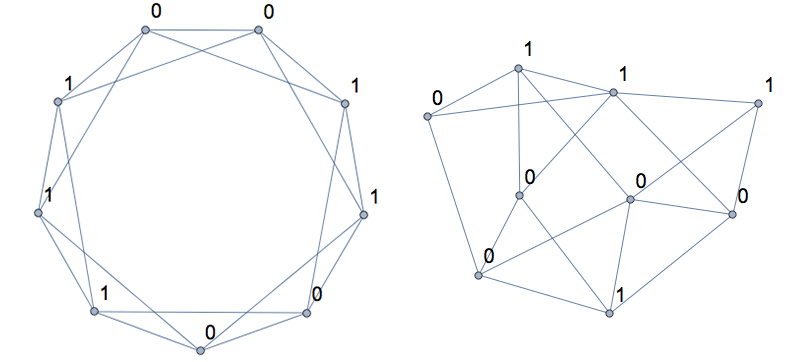
\includegraphics[width=\linewidth]{graphs.png}
\caption{(a) A graph with $n = 9$, $k = 4$ and (b) a graph with the same parameters but rewired with probability $e = 0.1$.}
\label{fig:graphing}
\end{figure}

\subsubsection{Paths}
\label{subsub:paths}

An update was carried out random-sequentially through the nodes, ie in each iteration a random path across the nodes was chosen and the states of each node were updated sequentially using a majority rule. Once all of the nodes had been updated (once each), a new random path was assigned and the nodes were once again updated, see Table \ref{tab:paths} below for an example. Updates were carried out dynamically: within an iteration node states were called as their neighbor was reached in the path, not once at the beginning; ie if node $5$'s state was changed to $1$ from $0$, the new state ($1$) is used for subsequent calculations involving node $5$ in the same iteration.

\begin{center} %centers table and caption in column
	\begin{minipage}{.7\linewidth} %use a minipage to compress the table caption
	\begin{table}[H]
		\centering %center the table within the minipage
		\renewcommand{\arraystretch}{1.3} %change \arraystretch in `tabular' to increase row height
		\caption{An example of random-sequential paths.}
		\label{tab:paths}
		\begin{tabular}{c | c} %two centered columns, separated by a vertical line
			Iteration & Path across nodes \\ \hline \hline %double horizontal line
			1 & 3 $\rightarrow$ 1 $\rightarrow$ 5 $\rightarrow$ 6 $\rightarrow$ 2  $\rightarrow$ 7 $\rightarrow$ 4 \\ \hline
			2 & 5 $\rightarrow$ 3  $\rightarrow$ 7 $\rightarrow$ 4 $\rightarrow$ 2 $\rightarrow$ 6 $\rightarrow$ 1 \\ \hline
			3 & 7 $\rightarrow$ 5 $\rightarrow$ 4 $\rightarrow$ 1 $\rightarrow$ 6  $\rightarrow$ 3 $\rightarrow$ 2 \\ \hline
		\end{tabular}
	\end{table}
	\end{minipage}
\end{center}

\vspace{0.5em} %add extra blank vertical space below matrix


\subsubsection{Majority Rule}
\label{subsub:majority}

The state of each node was updated using a majority rule with a threshold, $h \in [0.5, 1]$. A majority above the threshold, $h$, was required for the state of a node to be updated. See Table \ref{tab:majority} below.

\begin{center} %centers table and caption in column
	\begin{minipage}{.7\linewidth} %use a minipage to compress the table caption
	\begin{table}[H]
		\centering %center the table within the minipage
		\renewcommand{\arraystretch}{1.3} %change \arraystretch in `tabular' to increase row height
		\caption{An example of the majority rule with $h = 0.6$.}
		\label{tab:majority}
		\begin{tabular}{c | c | c} %three centered columns, separated by a vertical line
			Node value & Connected values & New value\\ \hline \hline %double horizontal line
			0 & 0, 0, 0, 1, 1 & 0 \\ \hline
			0 & 0, 0, 1, 1, 1 & 1 \\ \hline
			1 & 0, 0, 0, 1, 1 & 0 \\ \hline
		\end{tabular}
	\end{table}
	\end{minipage}
\end{center}


\subsection{Dissensus}
\label{sub:dissensus}

Dissensus was calculated using the committee size and the final population with state $0$, across all possible values of the initial population with  state $0$.  This gives

\begin{align}
\label{eq:dissensus}
D(N) \equiv \Biggl\langle \Theta \Biggl(1 - \frac{max(S_f, N - S_f)}{N}\Biggr)\Biggr \rangle_{S_i}
\end{align}

where $N$ is the committee size, $S_f$ the final population with  state $0$, $S_i$ the initial population with state $0$, $\langle \cdot \rangle_{S_i}$ the mean across all possible values of $S_i$, and $\Theta (x)$ the Heaviside step function ($0$ for $x = 0$ and $1$ for $x > 0$). 


\subsection{Data Collection}
\label{sub:datacollection}

Two forms of final data were collected: evolution plots displaying how the states of members changed through the iterations; and plots showing how dissensus varied with respect to $k$, $h$, $e$, and $N$.\par

The graphing methods were run with varying values of $k$, $h$, $e$, and $N$. For each of these dissensus was calculated $40$ times for each $S_i = 0, 1,... N$. From this the mean was calculated across all $S_i$, giving a value of $D(N)$ for a specific $k$, $h$, $e$, varying with $N$.

\section{Results and Analysis}
\label{sec:resultsanalysis}

A mean of all of the data obtained was measured, 

\section{Conclusion}
\label{sec:conclusion}

In conclusion, this template contains examples of some of the key features that might be found in a formal report created using \LaTeX. One more thing that's needed however is a list of armadillo species:

\begin{itemize} %start list
\item Banded Armadillos
\begin{enumerate} %start sub-list
	\item Seven-Banded
	\item Nine-Banded
\end{enumerate}
\item Airy Armadillos
\begin{itemize}
	\item Fairy Armadillos
	\begin{itemize}
		\item Greater Fairy
		\item Pink Fairy
	\end{itemize}
\end{itemize}
\end{itemize}

As you can see, there are lots of species of armadillo, some of which are nihilistic, but all of which are highly existential.

\begin{thebibliography}{99}
\label{references}

\bibitem{WikNi}
	R. L. Myer, ``Parametric oscillators and nonlinear materials,'' in \textit{Nonlinear Optics}, vol. 4, P. G. Harper and B. S. Wherret, Eds. San Francisco, CA: Academic, 1977, pp. 47-160.

\bibitem{WikAr}
	E. E. Reber et al., ``Oxygen absorption in the earth’s atmosphere,'' Aerospace Corp., Los Angeles, CA, Tech. Rep. Angeles, CA, Tech. Rep. TR-0200 (4230-46)-3, Nov. 1988.

\bibitem{WikMH}
	J. Jones. (1991, May 10). \textit{Networks} (2nd ed.) [Online]. Available: http://www.atm.com

\bibitem{NGRAM}
	 R. E. Kalman, ``New results in linear filtering and prediction theory,'' \textit{J. Basic Eng.}, ser. D, vol. 83, pp. 95-108, Mar. 1961.

\bibitem{NiMeme}
	J. P. Wilkinson, “Nonlinear resonant circuit devices,” U.S. Patent 3 624 125, July 16, 1990.


\end{thebibliography}


\appendix
\label{appendix}





\end{document}